\newpage
\subsection{QuizziPedia::Front-End::Filters}


\begin{figure} [ht]
	\centering
	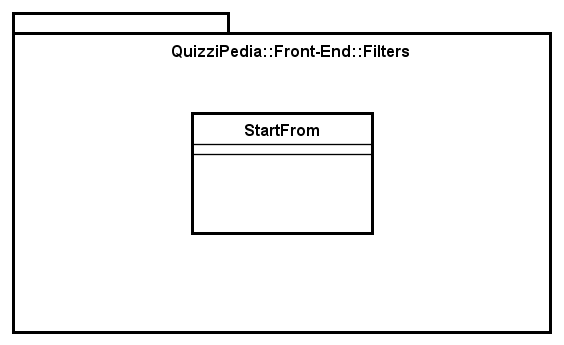
\includegraphics[scale=0.42]{UML/Package/QuizziPedia_Front-End_Filters.png}
	\caption{QuizziPedia::Front-End::Filters}
\end{figure} \FloatBarrier

\subsubsection{Informazioni generali}
\begin{itemize}
	\item \textbf{Descrizione}: 
	\item \textbf{Padre}: \texttt{Front-End};
	\item \textbf{Interazione con altri componenti}:
	\begin{itemize}
		\item \texttt{}:
	\end{itemize} 
\end{itemize}
\subsubsection{Classi}

\paragraph[QuizziPedia::Front-End::Filters::StartFrom]{QuizziPedia::Front-End::Filters::StartFrom}
\begin{figure} [ht]
	\centering
	\includegraphics[scale=0.80]{UML/Classi/Front-End/QuizziPedia_Front-end_Filters_StartFrom.png}
	\caption{QuizziPedia::Front-End::Filters::StartFrom}
\end{figure} \FloatBarrier
\begin{itemize}
	\item \textbf{Descrizione}: classe che permette di restituire una sezione di un array;
	\item \textbf{Utilizzo}: viene utilizzata per creare il meccanismo di visualizzazione in più pagine di una lista;
	\item \textbf{Relazioni con altre classi}:
	\begin{itemize}
		\item \textbf{OUT} \texttt{OneQuestionDirective}:rappresenta il componente grafico che visualizza all'utente l'anteprima della domanda che ha creato. Eseguendo l'azione di click sul pulsante di modifica sarà possibile modificare tale domanda. All'interno di \texttt{QuestionsManagementsView} verranno stampati a video tanti componenti quanti presenti nello \$scope isolato ad esso associato; 
		\item \textbf{OUT} \texttt{QuestionnaireDetailsDirective}: rappresenta il componente grafico che permette all'utente di visualizzare la lista di questionari che può compilare; 
		\item \textbf{OUT} \texttt{QuestionnaireDoneDetailsDirective}:; 
		\item \textbf{OUT} \texttt{SubscribeResultDirective}: rappresenta il componente grafico che permette all'utente di visualizzare la lista di questionari che ha già compilato e di conseguenza vederne le valutazioni; 
		\item \textbf{OUT} \texttt{UserResultsDirective}: directive che permette di visualizzare la lista degli utenti ricercati dopo aver utilizzato l'apposita funzione di ricerca; 
		\item \textbf{OUT} \texttt{CreateQuestionnaireView}: \textit{view\ped{G}} per la creazione del questionario; 
		\item \textbf{OUT} \texttt{RegistrationManagementView}: \textit{view\ped{G}} che permette di visualizzare gli utenti iscritti ad un questionario.
	\end{itemize}
	\item \textbf{Metodi}:
	\begin{itemize}
		\item \texttt{+} \texttt{startFrom()} \\
		Metodo costruttore della classe.
	\end{itemize}
\end{itemize}


